\documentclass[11pt]{article}
\usepackage{geometry}                % See geometry.pdf to learn the layout options. There are lots.
\geometry{letterpaper}                   % ... or a4paper or a5paper or ... 
%\geometry{landscape}                % Activate for for rotated page geometry
%\usepackage[parfill]{parskip}    % Activate to begin paragraphs with an empty line rather than an indent
\usepackage{graphicx}
\usepackage{amssymb}
\usepackage{epstopdf}
\usepackage{url}
\DeclareGraphicsRule{.tif}{png}{.png}{`convert #1 `dirname #1`/`basename #1 .tif`.png}

\title{XMLPipeDB User and Developer's Manual}
\author{The XMLPipeDB Group\\
Loyola Marymount University
}
%\date{}                                           % Activate to display a given date or no date

\begin{document}
\maketitle

\pagebreak
\tableofcontents
\pagebreak

\section{Overview}

XMLPipeDB is a suite of tools for managing, querying, importing, and exporting information to/from XML data based on some specific XML schema (XSD).  While its applicability is fairly general, the original motivation for XMLPipeDB is the management of biological data from different sources.  Thus, XMLPipeDB's end-user applications are bioinformatics-oriented, although other applications may be developed using the project's underlying tools.

\subsection{Who Should Read What Part of this Document}

\begin{itemize}
\item If you are a GenMAPP or other biological database user, you will want to read Section~\ref{endUserSoftware}.

\item If you are a bioinformatics software developer, you may also be interested in Sections~\ref{dblib}.

\item If you are a database administrator who is preparing an installation of one of XMLPipeDB's end-user applications, you will want to read Section~\ref{dbsetup}.

\item If you are a software developer or database designer who is interested in learning how XMLPipeDB's end-user applications were developed, you will want to read Section~\ref{devtools}.

\item Finally, if you are a software developer who wishes to participate in or contribute to the XMLPipeDB project, you will want to read Section~\ref{dev}.
\end{itemize}

\section{End-User Software}
\label{endUserSoftware}

\subsection{Pre-Built GenMAPP Files}

If your primary interest is to use GenMAPP for a particular organism, please consult the following list for GenMAPP files that have already been created using GenMAPP Builder (Section~\ref{genmappBuilder}).  In many cases, you can simply download them and point GenMAPP to them, and you'll be ready to load up expression data sets.

\begin{itemize}
\item E.\ coli K12
\item Pseudomonas putida
\item Bacillus subtilis
\end{itemize}

\subsection{GenMAPP Builder}
\label{genmappBuilder}

GenMAPP Builder is an application for creating files compatible with GenMAPP.  The application works by first importing supported data files into a relational database.  The database can then be queried by organism in order to produce a GenMAPP file.

\subsubsection{Usage}

To use GenMAPP Builder, you need:
\begin{itemize}
\item A Java 5 runtime environment
\item A relational database with an available JDBC 3 driver
\item One or more data sets downloaded from the Internet, from data sources that are currently supported by GenMAPP Builder
\end{itemize}
Once these are properly installed and operational, you can perform these primary functions:
\begin{enumerate}
\item Import one or more supported data files into the GenMAPP Builder database
\item Build a GenMAPP file based on an organism in the database
\end{enumerate}
The built files can then be read directly by GenMAPP.

\subsubsection{Supported Data Sets}
\label{supportedDataSets}

At this writing: UniProt and GO.

\subsubsection{Database Details}

GenMAPP Exporter performs the following specific details in generating a file that can be used by GenMAPP.  It is assumed that, upon, export:
\begin{enumerate}
\item Data has been loaded into the relational database used by GenMAPP Exporter (see Section~\ref{supportedDataSets} for details).

\item The specific items to be exported have been retrieved from the database by one or more queries.
\end{enumerate}
When the export command is invoked, GenMAPP Exporter does the following:
\begin{enumerate}
\item Create a blank GenMAPP Gene Database, consisting of the following four tables: \emph{Info}, \emph{Systems}, \emph{Relations}, and \emph{Other}.  This blank database comes from a template file in Microsoft Access format with extension .gtp.\footnote{In the program my student wrote at Vassar, I created a blank GenMAPP Gene Database from within GenMAPP using the Gene Database Manager and then this was used by the Exporter program.  The ``blank'' database starts out with the following four tables:  Info, Systems, Relations, Other.  If possible, it would be better to have the Exporter go ahead and create the database, adding these first four tables.}

\item Perform the MakeTable query to make the Uniprot systems table.\footnote{I need to look at what the fieldnames are in Uniprot so that I can tell you exactly what to grab.}

\item Make the other systems tables that can be derived from Uniprot cross-references: InterPro, Pfam, PDB, EMBL, TIGR CMR, EcoGene, EchoBase.

\item Make the ``Blattner'' systems table from the OrderedLocusNames field.

\item Make the relations tables between Uniprot and InterPro, Pfam, PDB, EMBL, TIGR CMR, EcoGene, EchoBase, and ``Blattner.''

\item Make indirect relations between TIGR CMR, EcoGene, EchoBase, and Blattner.\footnote{I'm pretty sure these should all be one-to-one relationships, but if we uncover instances where they are not, then we may have to abandon this.}

\item Make the OriginalRowCounts table, verifying that the tables are complete.\footnote{This might need to be a human step.  Somehow we need to verify, at least for Uniprot, that the number of records = the number of genes/proteins for that species.}

\item Edit the Info, Systems, and Relations tables so that they have the correct information to describe the database.\footnote{
At this point we would have a working GenMAPP Database, but without some ID systems that we would ultimately want and without Gene Ontology.

To add Gene Ontology to the database we could copy the GeneOntology, GeneOntologyCount, and GOTree tables from an existing GenMAPP database (these are the same for all) or we could work on making them ourselves.  Regardless of what we do for this, we will need to create Relations tables to Gene Ontology which means getting the data from somewhere.

For E. coli, we may need to use a special source (\url{http://www.genome.wisc.edu}).  For a generic solution, we will use the GOA project (another arm of the Uniprot people), \url{http://www.ebi.ac.uk/GOA/proteomes.html}.

We could find out if GOA matches the Wisconsin annotations for E. coli; if it does, we could just use GOA.

To be complete with all of the other species GenMAPP Databases, we should eventually grab data from NCBI's Gene Database.  \url{ftp://ftp.ncbi.nlm.nih.gov/gene}

And we should probably make a systems table for Affymetrix chip IDs.  This will be a little bit of a pain.}
\end{enumerate}

\section{Database Libraries}
\label{dblib}

The database libraries in XMLPipeDB are based, in turn, on the JAXB and Hibernate libraries.  To use these libraries in other software, you will need the following in your Java classpath:
\begin{itemize}
\item the database library itself (UniProtDB, GoDB, etc.)
\item Hibernate
\item JAXB
\item JDBC driver for your relational database
\end{itemize}
The libraries work like standard JAXB applications when importing XML files: the data in the loaded file gets converted into a set of corresponding objects.  The libraries then work like standard Hibernate applications when saving these objects to the database: configure Hibernate, then use its classes to save/update the objects or to perform HQL queries.

To further assist in software development, you may want to look at XMLPipeDB Utilities (Section~\ref{xmlpipedbutils}), which provide frequently-used routines and GUI components that are usually needed by applications using these libraries.

\subsection{UniProtDB}

UniProtDB is the library of Java classes that allows UniProt XML files to be transferred into a relational database.  The GenMAPP Exporter uses the UniProtDB library; in turn, the UniProtDB library is semi-automatically generated from the XMLPipeDB project's XSD-to-DB tool.

\subsection{GODB}

To be written\ldots

\section{Database Administration and Setup}
\label{dbsetup}

The applications in XMLPipeDB require any relational database for which a JDBC driver exists.  Thus, they all require some degree of configuration, for specifying the database server, database name, username, password, etc.  To facilitate this, XMLPipeDB includes a common database configuration GUI in all of its applications.

\section{Developer Tools}
\label{devtools}

Many components in XMLPipeDB's end-user applications are actually built semi-au\-to\-mat\-ic\-al\-ly.  The XMLPipeDB project includes these tools as well.  End-users don't need to know about these tools; instead, they use the \emph{output} generated by them.  This section is for database designers and software developers who are interested in creating their own XML-compatible database applications.

\subsection{XSD-to-DB}

The XSD-to-DB application takes a well-formed XML Schema (XSD) file and converts it into a collection of Java source code and Hibernate mapping files that allows XML files based on that XSD to be read into a relational database.  It was used to create the UniProtDB library which is used by GenMAPP Exporter.

XSD-to-DB's conversion functions are based on the open-source Hyperjaxb2 project (\url{https://hyperjaxb2.dev.java.net}).  It requires the following information to do its work:
\begin{itemize}
\item URL for the XML Schema (XSD) file to convert
\item Hyperjaxb2 binding file
\item Directory that will contain its output
\end{itemize}
XSD-to-DB comes with a default binding file, which it copies into its output directory when it is invoked for the first time.  Additional customization can then be performed on the copied binding file, and subsequent invocations of XSD-to-DB will use that binding instead of the default.

\subsubsection{Usage}

XSD-to-DB currently works as a command-line application, \texttt{xsd2db}.  If you invoke it without any arguments, XSD-to-DB will ask for the URL of the XSD file to convert.  Once the URL has been provided, XSD-to-DB then processes it produces Java source code, Hibernate mapping files, and an SQL DDL file that corresponds to the schema defined by the XSD file.  These files are placed in an output directory, which defaults to \texttt{db-gen} if it isn't otherwise specified.

XSD-to-DB behaves a little differently depending on the presence of certain files in the output directory, or even the presence of the output directory itself.  If the output directory is not present, then XSD-to-DB does the following:
\begin{enumerate}
\item Create the output directory.
\item Copy the XSD file from its given URL to the output directory.
\item Copy the default XSD-to-DB bindings file to the output directory.
\end{enumerate}
If the output directory already exists, then XSD-to-DB looks for the XSD and bindings files at the expected locations within that directory.  If those files are not present, then it performs the same steps as before.
\begin{itemize}
\item XSD-to-DB can be told whether or not to update the XSD file from its URL, in case the XSD file might have changed.  If it is told to perform an update, it will ask for the URL of the updated XSD file.
\end{itemize}
Once the output directory has been set up, XSD-to-DB then processes the XSD and bindings files to generate:
\begin{itemize}
\item Java source code for classes represented in the XSD
\item SQL DDL file defining the relational database tables that correspond to the Java classes
\item Hibernate mapping files that determine how the Java classes are convert to and from the relational tables
\item An Apache Ant \texttt{build.xml} file which can compile everything into a Java archive, ready for further development or deployment
\end{itemize}
From this point, a typical workflow would be:
\begin{enumerate}
\item Build a relational database using the generated SQL DDL file
\item Build the database library using the supplied Ant file, then use that library to test XML import, queries, and other database functions
\item Edit the bindings file to customize, correct, or improve the Java classes, Hibernate mappings, and relational tables generated from the XSD file
\item Re-run XSD-to-DB to actually create the new files
\end{enumerate}
Certain conversions might not be adequate even with extensive editing of the bindings file; in this case, the last resort is to manually edit the Java, Hibernate, and SQL files generated by XSD-to-DB.  If this is done, be careful about re-running XSD-to-DB on this particular output directory --- XSD-to-DB \emph{always} generates the Java, Hibernate, and SQL files ``from scratch,'' using the XSD and bindings files in the output directory.

Typically, once the generated files work as desired, the output directory becomes a software project in and of itself, to be edited, debugged, tested, and deployed like any other database library.  The fact that it was initially generated by XSD-to-DB merely indicates that some time was saved in creating this database library as compared to a manual Java-to-relational implementation of the XSD file.

\subsubsection{Output Details}

XSD-to-DB's output directory structure is shown in Figure~\ref{output}.  Directories are shown in boldface, and files are shown in italics.  Names in parentheses indicate placeholders for specific names that depend on the XSD being converted.

\begin{figure}[htbp] %  figure placement: here, top, bottom, or page
   \centering
   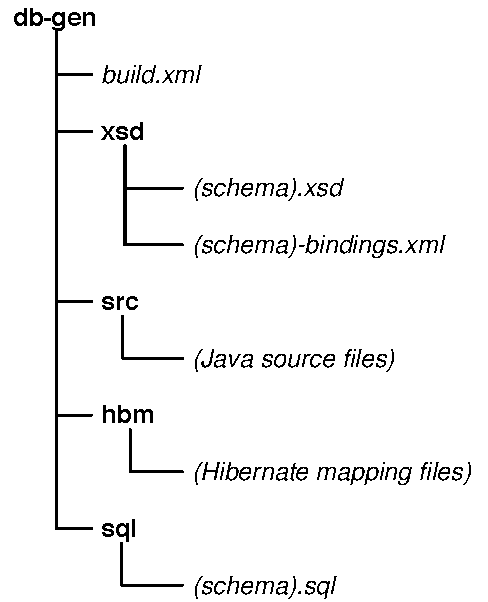
\includegraphics[width=2in]{figures/db-gen.pdf} 
   \caption{Structure of an XSD-to-DB output directory.}
   \label{output}
\end{figure}

The actual filenames and contents of terms in angle brackets $(< >)$ depend on the XSD file that was used to generate the output.  For instance, the UniProtDB library has \texttt{uniprot.xsd}, \texttt{uniprot-bindings.xml}, and \texttt{uniprot.sql}.

\subsubsection{Reference}

The \texttt{xsd2db} command line application accepts the following arguments:
\begin{description}
\item[\texttt{--outputDirectory=\emph{dir}}] The directory to use when generating (or re-generating) the database source code and files; defaults to \texttt{db-gen}.  Specifying a non-existent or empty directory essentially counts as a ``first-time run'' of XSD-to-DB.

\item[\texttt{--xsdURL=\emph{url}}] The URL for the XSD to convert; required when XSD-to-DB is run for the first time, or when \emph{updateXSD} (see below) is requested.

\item[\texttt{--bindings=\emph{filename}}] The bindings file to use when generating the database source code and files for the first time; this file is then copied into the \texttt{xsd} subdirectory.  Defaults to a standard bindings file supplied by XSD-to-DB.

\item[\texttt{-updateXSD}] Replaces the XSD being used with a new version; applicable only after XSD-to-DB has been run for the first time.

\item[\texttt{-help}] Displays a help message for how to use \texttt{xsd2db}.
\end{description}

\subsection{XMLPipeDB Utilities}
\label{xmlpipedbutils}

The XMLPipeDB Utilities library is a suite of Java classes that provide functions that are common to most XMLPipeDB database applications.  Specifically, the library includes reusable classes for:
\begin{itemize}
\item Loading of XML files into Java objects
\item Saving XML-derived Java objects to a relational database
\item Rudimentary query and retrieval of Java objects from the relational database
\item Configuring a client application to communicate with a relational database
\end{itemize}
XMLPipeDB Utilities includes a small GUI application that demonstrates these functions, using database code that was generated by XSD-to-DB.

By ``rudimentary query and retrieval,'' XMLPipeDB Utilities provides a facility for typing in an HQL (Hibernate Query Language) query coupled with an object browser that allows the user to examine the results of that query.  This is meant primarily for debugging or advanced purposes.

The library is separated into two layers: one layer provides the functionality, meant to be called programmatically, and another layer is a set of user interface components that allow end-user to invoke those functions.  Figure~\ref{utils} provides an overview of the library.

\begin{figure}[htbp] %  figure placement: here, top, bottom, or page
   \centering
   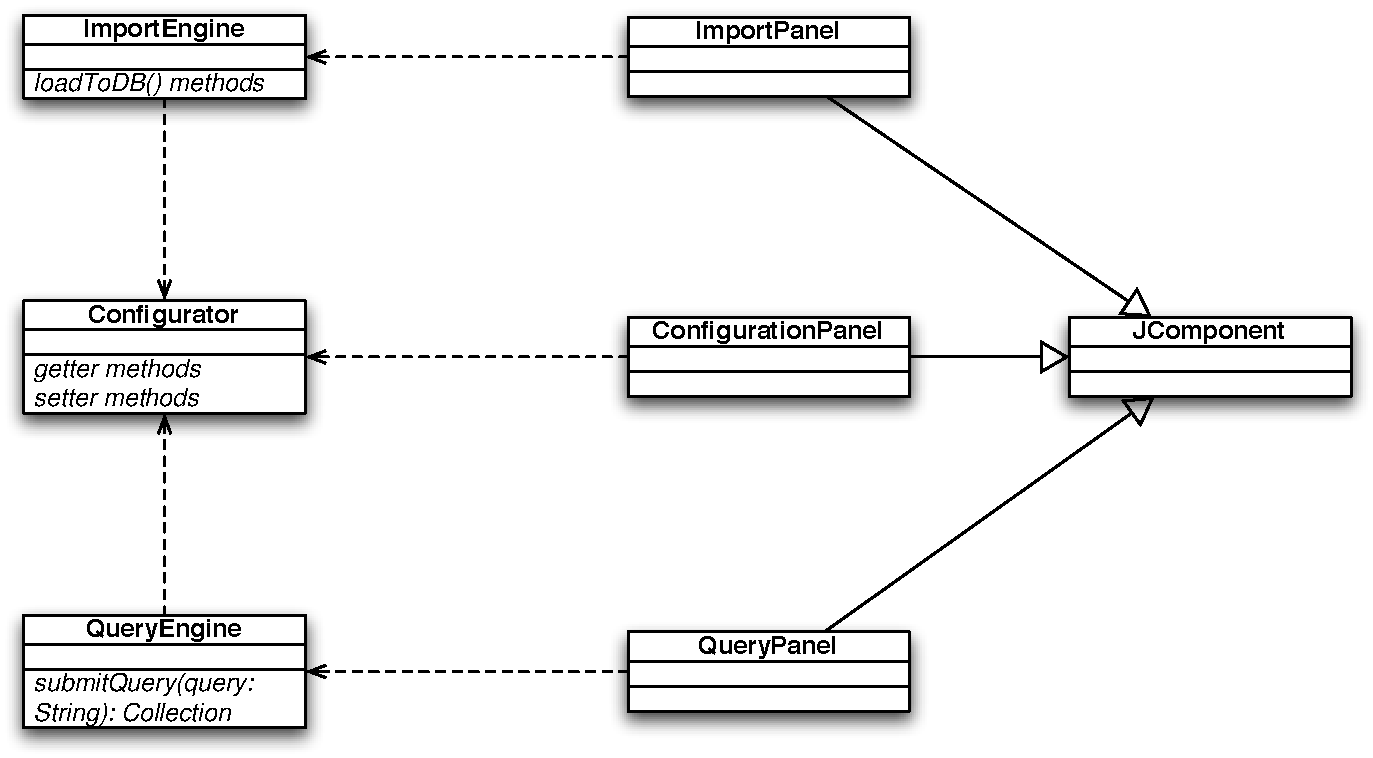
\includegraphics[width=5in]{figures/xmlpipedb-utilities.pdf} 
   \caption{Overview of XMLPipeDB Utilities.}
   \label{utils}
\end{figure}

\subsubsection{Utility Functions}

The following entities capture the functions provided by XMLPipeDB Utilities:
\begin{itemize}
\item \texttt{ImportEngine} provides a family of \emph{loadToDB()} functions, which takes any compliant file or input stream, parses them into their corresponding objects, then commits the objects to the database.

\item \texttt{Configurator} is the centralized location for configuration information used by XMLPipeDB.  It provides functions for retrieving, setting, and validating configuration properties.

\item \texttt{QueryEngine} is a generalized query wrapper whose \emph{submitQuery()} function takes a Hibernate query (in HQL, Hibernate Query Language) and returns the results as a Java collection.
\end{itemize}
Programs using the XMLPipeDB Utilities library can invoke these functions as necessary, using whatever mechanism is most appropriate for a particular application.

\subsubsection{User Interface Components}

To ease the development and delivery of these functions to end-user applications, XMLPipeDB Utilities also includes a component library that can be added directly into Java Swing windows and panels.  Each component provides a ``hook function'' that invokes the underlying operation, assuming that sufficient information has been gathered by the component:
\begin{itemize}
\item The \texttt{ImportPanel} family provides front-ends for database imports, displaying components like file choosers, text editors, and preview panels to make database loading as easy as possible for end-users.

\item The \texttt{ConfigurationPanel} family of components provides front-ends for the properties in \texttt{Configurator}.  The components are designed to be easily added to dialog boxes or preferences windows, and provide direct hooks to the \texttt{Configurator} functions.

\item The \texttt{QueryPanel} components allow users to enter HQL queries for submission to \texttt{QueryEngine}.  Correspondingly, a family of \texttt{ResultPanel} components provide reusable displays for the collections returned by \texttt{QueryEngine}.
\end{itemize}
The demo application that comes with XMLPipeDB Utilities shows how these components are used, and how they interact with the underlying functionality.

\section{Developer Documentation}
\label{dev}

\subsection{Use Case Model}

Figure~\ref{usecase} shows the use case model for the various components of the XMLPipeDB project.  These use cases are the basis for the activities described in this manual.

\begin{figure}[htbp] %  figure placement: here, top, bottom, or page
   \centering
   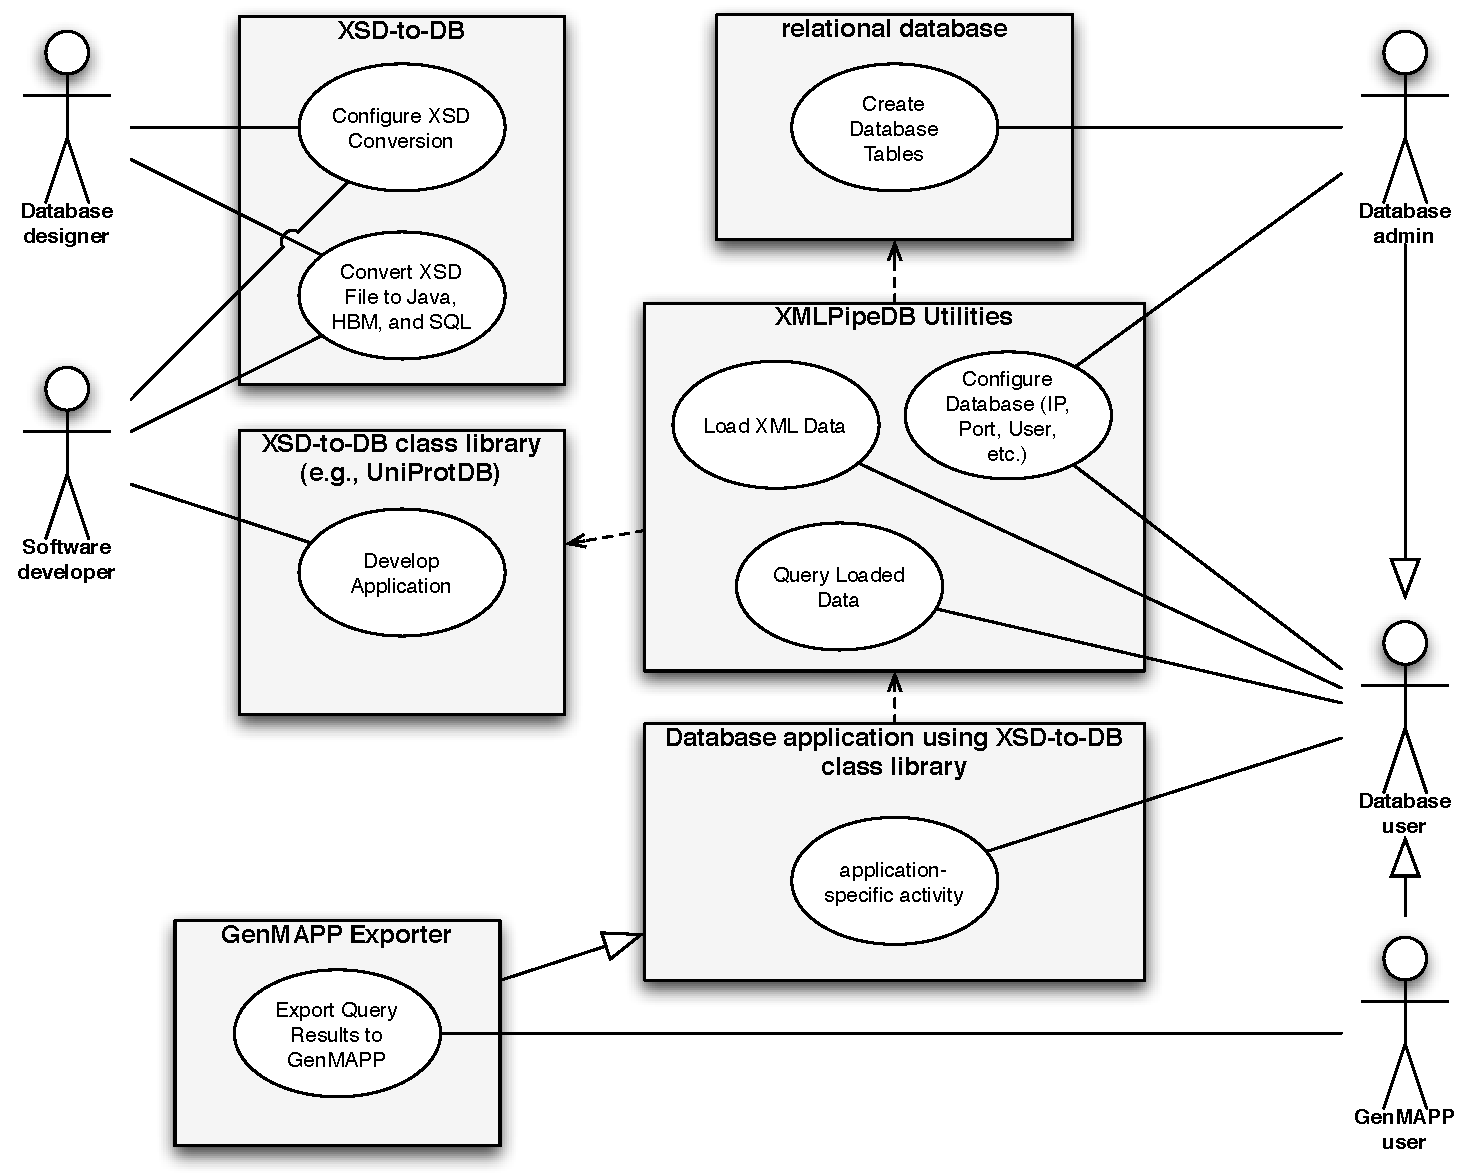
\includegraphics[width=5.5in]{figures/use-cases.pdf} 
   \caption{Use case model for the XMLPipeDB project.}
   \label{usecase}
\end{figure}

\subsection{Guide to the Repository}

The XMLPipeDB project consists of a number of modules, listed hierarchically in Figure~\ref{cvs}.  They are related but intended to be standalone.

\begin{figure}[htbp] %  figure placement: here, top, bottom, or page
   \centering
   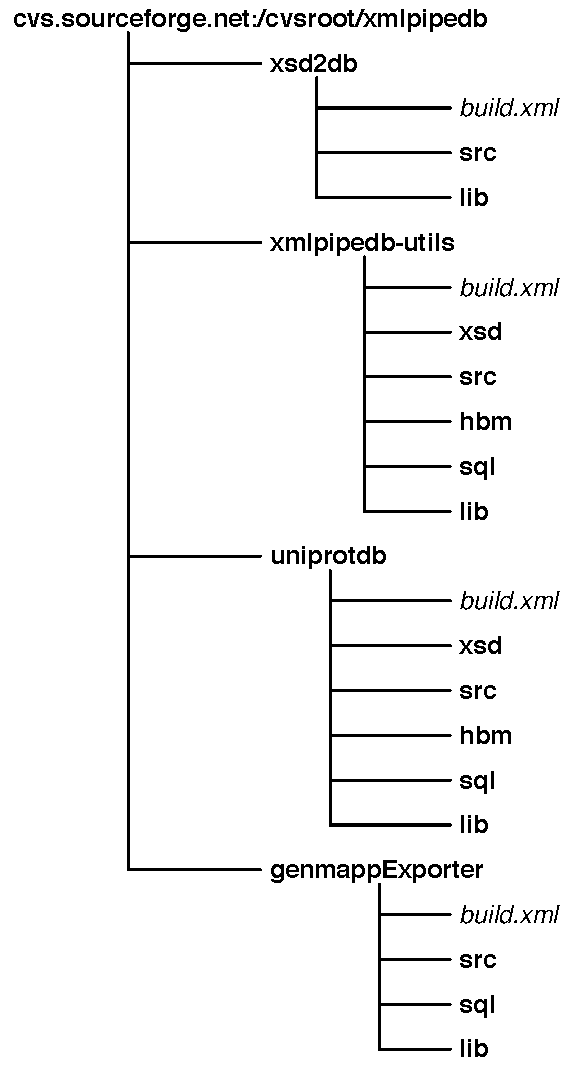
\includegraphics[width=2.5in]{figures/cvs.pdf} 
   \caption{Structure of the XMLPipeDB CVS repository.}
   \label{cvs}
\end{figure}

The \texttt{xsd2db} module contains the source code and libraries to XSD-to-DB.  XMLPipeDB Utilities resides in the \texttt{xmlpipedb-utils} module, including the source for its demo application.  When it is built, XMLPipeDB Utilities separates its reusable component (\emph{xmlpipedb-utils.jar}) from the demo application that uses it (\emph{xmlpipedb-utils-demo.jar}).

The sources for the UniProtDB library, which was generated by XSD-to-DB then manually customized, resides in the \texttt{uniprotdb} module.  Finally, the source code to the GenMAPP Exporter application resides in the \texttt{genmappExporter} module.  Each module contains an Apache Ant \texttt{build.xml} file that can compile the source into distributable binaries; these build products are placed in the \texttt{dist} subdirectory, and should not be committed to the repository.

Similarly, output produced by XSD-to-DB (which defaults to \texttt{db-gen} in the current working directory at the time XSD-to-DB is invoked) should be committed as new modules in the repository, such as with \texttt{uniprotdb}.  Of course, the default \texttt{db-gen} name should be changed to something more descriptive.

\subsection{Building from Source}

As mentioned, building fresh binaries of each XMLPipeDB module is a matter of downloading or checking out the source then invoking Apache Ant in each module's top-level directory.  Build products are placed in the \texttt{dist} subdirectory, and should not be committed to the repository.

\subsection{Unit Tests}

We need them\ldots'nuff said!

\subsection{Third-Party Libraries}

XMLPipeDB ``stands on the shoulders'' of a wide variety of third-party libraries.  These libraries are always stored in the \texttt{lib/} subdirectories of each XMLPipeDB module.  Most of these third-party libraries are themselves active open source projects that continue to be developed; thus, to avoid confusion and accidental incompatibilities, all third-party libraries committed to XMLPipeDB are appended with a version number.  For example, if an XMLPipeDB module uses Jakarta Commons Logging 1.0.4, then \texttt{-1.0.4} is appended to the standard library name, so that it is stored in \texttt{lib/} as \texttt{commons-logging-1.0.4.jar}.

If a third-party library is to be updated with a new version --- and of course this new version has been verified to work with the existing code --- then its prior version should be deleted and a new file added with the appropriate version suffix.

\end{document}
